A pesquisa desenvolvida nesta monografia investiga e elabora uma solução voltada para organização
de uma coleção de documentos textuais de maneira flexível. O processo de organização em si, conforme 
discutido ao longo dos capítulos, envolve uma gama de desafios para ser executado com eficiência, como, 
por exemplo, os impactos negativos da elevada dimensionalidade da matriz documentos x termos, que 
é comumente muito esparsa em coleções textuais. Por conta disso, a tarefa de se calcular a similaridade
entre dois documentos quaisquer, a partir daquela mesma matriz, apresenta alto grau de dificuldade. 
Outro problemática fundamental está no processo de agrupamento, através do qual se espera que os grupos resultantes 
consigam capturar a estrutura natural das coleções e que esses grupos possuam relevância para os usuários finais. 
Atendendo a esses princípios, o agrupamento consegue cumprir o papel de aquisição e descoberta de conhecimento. Coleções textuais podem também 
conter documentos ruidosos, que destoam do restante da coleção, sendo que é esperado o emprego de técnicas no processo de organização
flexível para que ele não seja prejudicado pela presença desses documentos. Com o aumento massivo da
quantidade de dados produzidos pela humanidade, se faz também necessário que todo o processo seja
capaz de se adequar a coleções com grande volumes de dados. Assim, a organização flexível de documentos proposta fundamenta-se em um conhecimento 
bastante intensivo, por meio do qual se aplica um conjunto de diversas técnicas os desafios apontados acima bem como outros associados a 
esse processamento de textos. Parte relevante das técnicas aqui empregadas derivam dos estudos demineração de textos e, consequentemente, 
também da mineração de dados. 

Todo esse contexto apresentado se mostra inviável de ser abordado de maneira aprofundada em uma única
pesquisa. Por isso, as investigações conduzidas nessa monografia foram focadas no aumento da
robustez do processo, reduzindo-se os impactos dos dados ruidosos ao se utilizar uma estratégia
híbrida com o algoritmo PFCM. Portanto, a hipótese formulada e verificada nesta monografia foi:

\begin{quote}
\textit{A utilização de uma estratégia híbrida de agrupamento e extração de descritores, entre os 
  graus de pertinência e tipicidade providos pelo método de agrupamento PFCM, permitem o aumento da
    robustez e resiliência contra ruídos na organização flexível de documentos, aumentando assim a
    relevância dos grupos obtidos.}
\end{quote}

Portanto, com base na exploração das estratégias existentes na literatura para aprimoramento do
processo de organização flexível de documentos e da avaliação da hipótese formulada, o objetivo
desta monografia é definido como segue:

\begin{quote}
\textit{Conduzir uma investigação em torno dos métodos de agrupamento FCM, PCM e PFCM, para
se compreender e interpretar corretamente as peculiaridades de se extrair descritores em um
agrupamento híbrido.}
\end{quote}

A fim de atender a esse objetivo, foi realizado nesta monografia um estudo dos fundamentos
necessários para a organização flexível de documentos, uma revisão das estratégias recentes
utilizadas por pesquisadores para aprimorar a organização flexível de documentos. E, por fim, como
resultado, o estudo dos impactos de se utilizar o algoritmo PFCM no processo e na extração de
descritores, o qual derivaram a proposição de dois métodos de extração de descritores: PDCL e
Mixed-PFDCL. Tais métodos são extensões do método SoftO-FDCL apresentado em \cite{Nogueira2013}, e
diante dos resultados, contribuem de maneira significativa para o estado da arte da extração de
descritores dos grupos fuzzy.

Na seção seguinte, apresentam-se as principais contribuições fornecidas por esta monografia e os
possíveis trabalhos futuros que derivam desta pesquisa.

\section{Resumo das contribuições}

A investigação realizada nesta monografia, produziu algumas importantes contribuições para o
processo de se organizar documentos de maneira flexível. Essas contribuições são distribuídas no estudo e
fundamentação da teoria relacionada a esse campo de estudo, investigação e apresentação das
possibilidades de aprimoramento e otimização do processo explorados recentemente na literatura e a
investigação das peculiaridades de adotar uma estratégia híbrida o que posteriormente motivou a
proposição de dois métodos de extração de descritores. 

A partir do estudo da teoria e dos fundamentos necessários para o tema, é apresentado nesta
monografia um rico conteúdo abordando os detalhes dos métodos de agrupamento FCM, PCM, PFCM e HFCM,
juntamente com os seus pseudo-códigos, para auxiliar novos pesquisadores na rápida implementação de
tais métodos.

Outra importante contribuição, consiste na apresentação das pesquisas que se situam no estado da
arte das etapas presentes no processo de organização flexível de documentos. Ficou evidenciado, a
partir das pesquisas encontradas na literatura, a diversidade as estratégias existentes na literatura
para mitigar os desafios existentes. Foi visto que ainda é proposto abordagens para aprimorar todas
as etapas existentes no processo, as quaiscontemplam o pré-processamento, agrupamento, extração
de descritores e recuperação da informação, com isso conclui-se que a organização flexível não é um
problema resolvido na literatura, o que o torna um problema de pesquisa bastante promissor. 

A primeira contribuição experimental dessa monografia, consistiu no estudo dos impactos de se
adicionar o método PFCM no processo de organização flexível de documentos. A partir desse estudo
foi observado que o algoritmo PFCM possui uma tendência para aumentar a eficiência do
agrupamento produzido em coleções textuais de maior dimensionalidade, o que foi comprovado a partir
das evidências contidas na Tabela \ref{table:pfcmsummary}. No entanto, se destaca aqui a importância
da realização de novos estudos com um maior número de coleções textuais de baixa e alta
dimensionalidade para se confirmar esta tendência. 

Por outro lado, constatou-se nesse experimento a capacidade de adaptação do método
SoftO-FDCL a novos algoritmos de agrupamento. No entanto, este último método, segundo as suas pesquisas iniciais, considera somente uma única
partição no processo de pontuação dos termos candidatos, o que por sua vez não consegue capturar
toda a essência do agrupamento produzido pelo PFCM. Ainda nesse experimento foi observado um
problema na interpretação das tipicidades contidas em partições possibilísticas, no processo de
extração de descritores. Esse problema deriva diretamente da natureza probabilística dos graus de
pertinência da partição fuzzy do FCM, que não se aplica às tipicidades, a qual influencia
direta adequação ou não do limiar $\delta$ do método SoftO-FDCL. 

Portanto, a partir da identificação desse problema de interpretação dos graus de compatibilidade
possibilísticos, uma outra importante contribuição dessa monografia, consiste na formulação das
propriedades do limiar apresentadas nas equações \ref{eq:limiarp1}, \ref{eq:limiarp2} e
\ref{eq:limiarp3}. Essas propriedades expressam características importantes, que os graus de
compatibilidade devem possuir, para o limiar $\delta$ do método do método SoftO-FDCL conseguir
extrair bons descritores dos grupos. 

Feitas essas considerações, apresentam-se as duas principais contribuições dessa monografia. A primeira consiste no
método PDCL, que propõe uma abordagem para interpretar os graus de compatibilidade possibilísticos,
respeitando as propriedades das equações \ref{eq:limiarp1}, \ref{eq:limiarp2} e \ref{eq:limiarp3},
sem deixar de lado a resiliência contra ruídos inerente das tipicidades. Os experimentos conduzidos
com esse método demonstraram a qualidade dos descritores extraídos com o PDCL em comparação com o
método SoftO-FDCL, cujos comparativos estão apresentados na Tabela \ref{table:rankingpdcl}. No entanto, observou-se
neste experimento que o método PCM produziu uma quantidade baixa de grupos em comparação ao número
total de classes em cada coleção, assim como também a defuzificação resultou em grupos majoritários
com elevado percentual. Com isso, é importante salientar, a necessidade de se conduzir estudos
experimentais a respeito dos parâmetros ideais dos métodos de agrupamento para coleções textuais.

A segunda grande contribuição desta monografia consiste na proposta de um método de extração de
descritores híbrido, capaz de interpretar as duas partições presentes no algoritmo PFCM de maneira
bastante satisfatória. Um segundo experimento foi então conduzido para atestar os
benefícios desse abordagem híbrida de extração de descritores. Os resultados apresentados no sumário
da Tabela \ref{table:pdclsummary}, atestam através de uma avaliação preditiva com clássicos
algoritmos de classificação, que os descritores extraídos através do método Mixed-PFDCL no
agrupamento resultante do método PFCM, foram melhores que os descritores do método SoftO-FDCL.
Ainda na Tabela \ref{table:rankingmixedpdcl}, se demonstrou que os descritores obtidos com o método
Mixed-PFDCL preservam uma proximidade semântica, com os demais termos do mesmo grupo, assim como os
descritores do método SoftO-FDCL.

Durante as pesquisas realizadas neste projeto de conclusão de curso, houve a publicação de um artigo
com os resultados obtidos no primeiro experimento, em uma das mais importantes conferências de
sistemas fuzzy. Isso reforça a importância e relevância do tema estudado nesta monografia para a
comunidade científica. Segue o artigo publicado:
\begin{quote}
CARVALHO, N. V. J. et al. Flexible Document Organization by Mixing Fuzzy and Possibilistic
Clustering algorithms. IEEE International Conference on Fuzzy Systems (FUZZ- IEEE), p. 1–8, 2016.
\end{quote}

\section{Trabalhos futuros}

Ao considerar todas as conclusões apresentadas anteriormente, existem diversas possibilidades que
podem derivar deste trabalho. Em particular, foi notado que é necessário se realizar uma avaliação
mais apurada dos impactos na variação dos parâmetros dos algoritmos de agrupamento, de modo que se
possa obter, senão uma forma automatizada dos parâmetros com base nas características das bases,
pelo menos indicações de quais parâmetros utilizar. 

Nesse sentido, está apresentado na Figura \ref{fig:pfcmvarying}, um exemplo dos impactos da variação
da quantidade de grupos e do parâmetro $m$, sobre a medida de silhueta fuzzy. Ao analisar o gráfico,
observa-se uma clara tendência da medida de silhueta fuzzy (FS) aumentar, com o incremento no número
de grupos e para a faixa de valores de $m$ entre 1,0 e 1,4. Contudo, esse tipo de análise requer
sucessivas execuções de todo o agrupamento, o que por sua vez é um processo bastante oneroso
computacionalmente. Sendo assim, pretende-se estender esse estudo para outras bases e para os
demais algoritmos de agrupamento, assim como mensurar a qualidade do agrupamento produzido
através de outras medidas de validação existentes na literatura, como, por exemplo, as medidas de
entropia e pureza do agrupamento apresentadas em \citeonline{Deepa2012} ou a medida de validação
proposta em \citeonline{ZhangZhou2008}, que explora as pertinências e tipiciadades existentes no
PFCM.

\begin{figure}[!h] \centering 
  \centering
  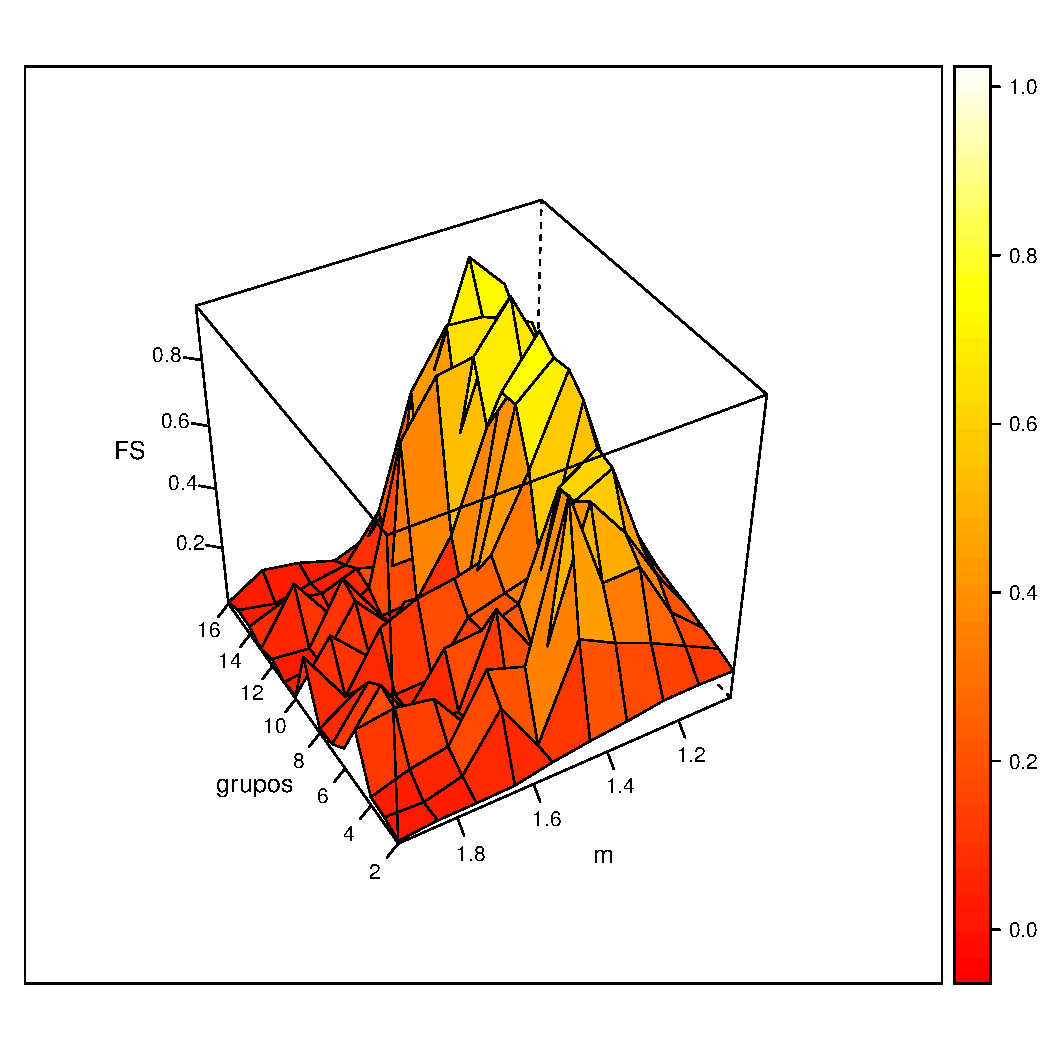
\includegraphics[width=0.8\columnwidth]{assets/future_works/pfcm_nsf_varying.pdf} 
  \caption{Gráfico das influências da variação da quantidade de grupos e do parâmetro $m$, na
pontuação obtida pela medida de silhueta fuzzy para o algoritmo PFCM na base NSF} 
  \label{fig:pfcmvarying}
\end{figure}

Nesta monografia, também foi observado diversas vezes que um dos grandes desafios no agrupamento de
documentos está na dimensionalidade dos dados. Soma-se a isso o fato de que os principais algoritmos
de agrupamento possuem como ponto crítico de decisão no processo de separação dos elementos em
grupos, a medida de similaridade. Sendo assim, é importante se investigar também as possibilidades de
aprimoramento da organização flexível de documentos com as recentes medidas de similaridade
propostas na literatura \cite{Lin2014,Nagwani2015} para dados de alta dimensionalidade e em
particular para coleções textuais.

Outro aspecto de grande relevância é a escalabilidade da proposta de organização flexível de
documentos, para coleções textuais que se enquadram na categoria {\it Very Large\/} de acordo com a
Tabela \ref{table:datasize}. Portanto, se pretende realizar estudos objetivando escalar o processo
utilizado nesta pesquisa para o cenário de {\it Big Data\/}, utilizando como base as pesquisas com
grandes quantidades de dados apresentadas em \citeonline{Honda:2014}, \citeonline{Wang:2014} e
\citeonline{Havens2012}. De antemão, postula-se que, no que diz respeito a implementação dos algoritmos
aqui utilizados, todo o processo deve ter sido paralelizado utilizando o framework de computação paralela
OpenMP ({\it Open Multi-Processing\/})\footnotemark, o que habilita a realização de experimentos em
computadores com elevado potencial de processamento.
\footnotetext{\url{http://openmp.org/}}

